\documentclass[11pt]{article}
\usepackage[margin=1in]{geometry}
\usepackage{amsmath,amssymb,amsthm,graphicx,booktabs,enumitem,float,tabularx,array}
\usepackage[hidelinks]{hyperref}
\usepackage[font=small,skip=3pt]{caption}
\setlength{\parindent}{0pt}
\setlength{\parskip}{0.3em}
\setlist{topsep=1pt,itemsep=1pt,parsep=0pt}
\setlength{\textfloatsep}{7pt}
\setlength{\floatsep}{6pt}
\setlength{\intextsep}{6pt}
\newtheorem{theorem}{Theorem}
\newtheorem{proposition}[theorem]{Proposition}
\newtheorem{lemma}[theorem]{Lemma}
\newcommand{\R}{\mathbb{R}}
\newcommand{\E}{\mathbb{E}}
\newcommand{\ip}[2]{\langle #1,#2\rangle}
\newcommand{\op}{\mathrm{op}}
\newcommand{\Gh}{\widehat G}
\newcommand{\err}{\mathrm{err}}
\newcommand{\Sh}{\mathcal S}
\DeclareMathOperator{\tr}{tr}
\makeatletter
\newcommand\tabin[1]{\@@input #1.tex }
\renewcommand\section{\@startsection{section}{1}{\z@}{-1.3ex plus -.3ex}{0.5ex}{\normalfont\large\bfseries}}
\renewcommand\subsection{\@startsection{subsection}{2}{\z@}{-1.0ex plus -.2ex}{0.3ex}{\normalfont\normalsize\bfseries}}
\makeatother

\begin{document}
{\small Optimization for Data Science, Autumn 2026 --- Final report \hfill [team names]}
\vspace{-0.4em}
\begin{center}
{\Large\textbf{Can a prior shrink the variance of EGGROLL?}}\\[0.25em]
{\large A low-rank prior, a sharp threshold, and why a better estimate need not train faster}
\end{center}
\vspace{-0.6em}

\section{Question and motivation}
Evolution strategies (ES) train a model from loss values alone, with no backpropagation. The EGGROLL method~[1] makes ES practical for models with billions of parameters. To update a weight matrix $W\in\R^{m\times n}$, it draws $N$ random low-rank matrices $E_1,\dots,E_N$ (\emph{probes}), measures the slope of the loss $f$ along each probe, and averages:
\begin{equation}\label{eq:es}
\Gh=\frac1N\sum_{j=1}^Ny_jE_j,\qquad y_j=\frac{f(W+\sigma E_j)-f(W-\sigma E_j)}{2\sigma}\approx\ip{E_j}{G},\qquad G=\nabla f(W).
\end{equation}
Each probe costs two forward passes, so $N$ is limited. The estimate $\Gh$ is unbiased on quadratics, but its relative error $\E\|\Gh-G\|^2/\|G\|^2$ is about $d/N$, where $d$ is the number of parameters~[2]. In practice $N\ll d$, so $\Gh$ is mostly noise (Figure~\ref{fig:idea}b).

Statistics has a standard remedy for a noisy estimate: \emph{shrinkage}. A prior or a penalty pulls the estimate toward a plausible structure and uses no new data, so here it costs no new forward pass.

\par\smallskip\noindent\hfil\begin{minipage}{0.93\textwidth}
\textbf{Question.} \emph{Can a prior or a penalty on the gradient reduce the error of the ES estimate \eqref{eq:es} with the same $N$ loss evaluations? If so, does the better estimate make ES training faster?}
\end{minipage}\par\smallskip

The answer is not obvious. The simplest shrinkage, a scalar factor $a\Gh$, is only a change of stepsize (our earlier notes~[N]). But gradients of neural networks are often close to low rank~[3, 12, 13]. Figure~\ref{fig:idea} shows how a prior can use this: the ES noise is spread evenly over all directions, so a low-rank gradient stands out in the \emph{singular values} even when every entry is dominated by noise. Table~\ref{tab:answers} lists our answers; the last one is negative.

\begin{figure}[!htb]
\centering
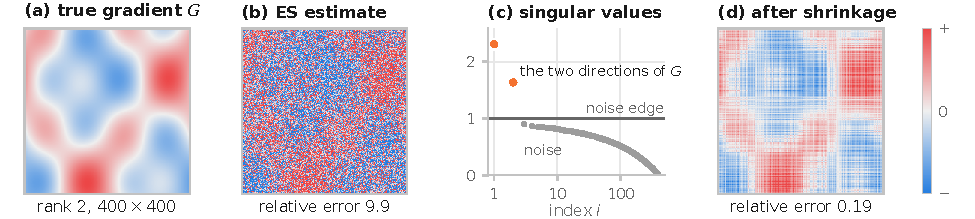
\includegraphics[width=\textwidth]{fig_idea.pdf}
\caption{The idea. (a) A rank-2 gradient. (b) Its EGGROLL estimate \eqref{eq:es} from $N=16000$ rank-one probes ($d/N=10$). (c) Singular values of (b) over the noise edge computed by Algorithm~1 (Section~\ref{sec:q2}): the two directions of $G$ stand out. (d) Algorithm~1 keeps and shrinks them, with no new loss evaluation.}\label{fig:idea}
\end{figure}

\begin{table}[!htb]
\centering\small
\caption{Our answers ($g$: whole gradient; $s_1$, $k$: top singular value and rank of an $m\times n$ layer gradient).}\label{tab:answers}
\begin{tabularx}{\textwidth}{@{}l>{\raggedright\arraybackslash}p{0.355\textwidth}>{\raggedright\arraybackslash}Xl@{}}
\toprule
 & Question & Answer & Result\\
\midrule
Q1 & Does a prior with no preferred direction help? & No: every estimator has relative error $\ge1-N/d$. & Thm.~\ref{thm:nogo}\\
Q2 & Does a low-rank prior help? & Yes, above a threshold $N^\star=\sqrt{mn}\,\|g\|^2/s_1^2$; the layer error then falls by up to $mn/(k(m+n))$. & Thm.~\ref{thm:spike}, \ref{thm:risk}\\
 & \dots\ with rank-one probes (EGGROLL)? & Yes, with 2 to 2.5 times more probes. & Prop.~\ref{prop:cov}\\
Q3 & Does the better estimate train faster? & Only if $N^\star<N\lesssim T$ (a curvature ratio); in our network, no. & Prop.~\ref{prop:ceiling}\\
\bottomrule
\end{tabularx}
\end{table}

\section{Related work and formulation}
\textbf{ES and zeroth-order methods.} Sarkar et al.~[1] introduce EGGROLL. Kaya and Hashemi~[2] show that the error of \eqref{eq:es} is $(d+1)/N$ for dense Gaussian probes, almost the same for low-rank probes, and half of it with a leave-one-out baseline. Other zeroth-order methods exploit sparse gradients~[8, 9], learned subspaces~[10, 11] or low-rank probes~[12, 13]. MeZO~[14] explains why zeroth-order fine-tuning works at all: the Hessian has low effective rank.

\textbf{Closest work.} Allen et al.~[3] (September 2026) treat the $y_j$ as linear measurements of the gradient matrix. For one matrix, dense Gaussian probes and a known rank $k$, matrix-sensing algorithms~[6, 7] recover an approximately rank-$k$ gradient from about $c\,k(m+n)$ probes, which speeds up optimization on synthetic functions whose gradients are low-rank everywhere. Without a rank assumption they use the pseudoinverse, the projection of $G$ on the span of the probes. We differ in four ways. (i) [3] designs solvers for $N\gtrsim k(m+n)$; we analyze the cheapest use of a low-rank prior, one SVD of the standard estimate \eqref{eq:es}, for \emph{every} $N$, and get an exact error curve with a sharp threshold. (ii) We treat EGGROLL's setting, which [3] leaves open: rank-one probes and many matrices that share each scalar. (iii) We show that without structure nothing beats their pseudoinverse. (iv) We ask when a better estimate speeds up descent at all.

\textbf{Setting.} The parameters are matrices $W_1,\dots,W_L$, $W_l\in\R^{m_l\times n_l}$, with $d=\sum_lm_ln_l$ entries. Let $g=(G_1,\dots,G_L)$ be the gradient at the current point, $\|g\|^2=\sum_l\|G_l\|_F^2$. A probe is $E_j=(E_{j,1},\dots,E_{j,L})$; as in EGGROLL, all layers share one scalar per probe. We assume:
\begin{itemize}[leftmargin=2.6em]
\item[(A1)] \emph{Exact slopes:} $y_j=\ip{E_j}{g}=\sum_l\ip{E_{j,l}}{G_l}$, $j=1,\dots,N$. (True for \eqref{eq:es} on a quadratic $f$ for every $\sigma$~[2, D]; the error is $O(\sigma^2)$ for a smooth $f$.)
\item[(A2)] \emph{Probes} are independent of $g$, and either \emph{dense} (i.i.d.\ $N(0,1)$ entries) or \emph{rank-$r$} ($E_{j,l}=AB^\top/\sqrt r$ with i.i.d.\ $N(0,1)$ entries in $A$, $B$; EGGROLL uses $r=1$).
\end{itemize}

\textbf{Estimators.} An \emph{estimator} is any function $\tilde g$ of the data $(E_j,y_j)_{j\le N}$. The ES estimate is $\hat g=\frac1N\sum_jy_jE_j$, with layers $\Gh_l$. The \emph{relative error} is $\err(\tilde g)=\E\|\tilde g-g\|^2/\|g\|^2$ (likewise for one layer); $\err(0)=1$, and $\err(\hat g)=(d+1)/N$ for dense probes.

\textbf{Shrinkage.} A penalty $\mathrm{pen}$, which plays the role of the negative log-density of a prior, defines $\tilde g=\arg\min_h\frac12\|h-\hat g\|^2+\mathrm{pen}(h)$. The ridge penalty $\frac\lambda2\|h\|^2$ gives the scalar shrinkage $\hat g/(1+\lambda)$. A penalty on the singular values of a layer, such as the nuclear norm, gives \emph{singular-value shrinkage}: $\Sh(\Gh)=\sum_i\eta(\hat s_i)\,\hat u_i\hat v_i^\top$, where $\Gh=\sum_i\hat s_i\hat u_i\hat v_i^\top$ is the SVD of the layer estimate and $0\le\eta(s)\le s$.

\textbf{Three precise questions.} For one layer we write $G\in\R^{m\times n}$ with $m\le n$, $\beta=m/n$, singular values $s_1\ge s_2\ge\dots$, and $\nu=\|g\|/\sqrt N$.
\begin{itemize}[leftmargin=2.6em]
\item[(Q1)] If nothing is known about the direction of $g$, how small can the error of an estimator be?
\item[(Q2)] If $G$ has a few large singular values, what is the error of $\Sh(\Gh)$, for which $N$ is it below $1$, and what changes for rank-one probes?
\item[(Q3)] For a quadratic $f$ with Hessian $H$, a step along $U$ decreases $f$ in expectation by at most $\Delta(U)=\max_\eta\E[f(W)-f(W-\eta U)]=(\E\ip{g}{U})^2/(2\,\E\ip{U}{HU})$. How much larger is $\Delta$ for a better estimate than $\hat g$?
\end{itemize}

\section{Approach and results}
Theorems~\ref{thm:nogo}, \ref{thm:spike}, Proposition~\ref{prop:cov} and all experiments are ours. Theorem~\ref{thm:risk} combines Theorem~\ref{thm:spike} with known limits~[4, 5], and Proposition~\ref{prop:ceiling} is an exact form of the analysis of~[14]. Proofs: Appendix~\ref{app:proofs}.

\subsection{Q1: a prior without a preferred direction cannot help}
\begin{theorem}[No gain without structure]\label{thm:nogo}
Assume (A1), probes of any law that are independent of $g$, and $N<d$. If the direction of $g$ is uniformly random (any rotation-invariant law with $\E\|g\|^2=1$), then every estimator satisfies $\E\|\tilde g-g\|^2\ge1-N/d$. Hence $\max_{\|g\|=1}\err(\tilde g)\ge1-N/d$.
\end{theorem}
\emph{In words:} $N$ probes reveal $N$ coordinates of $g$ in a suitable basis and nothing about the rest. The pseudoinverse of~[3] attains the bound, and the best multiple of the ES estimate is as good when $N\ll d$ (Appendix~\ref{app:proofs}). So ridge, James--Stein, or any prior without a preferred direction gains nothing beyond a change of stepsize~[N]. \emph{A useful prior must prefer some directions.}

\subsection{Q2: a low-rank prior helps above a sharp threshold}\label{sec:q2}
\begin{theorem}[The ES estimate is the gradient plus white noise]\label{thm:spike}
Assume (A1) and dense probes. For every $g\ne0$, with $u=g/\|g\|$,
\[
\hat g\ \overset{d}{=}\ \alpha\,g+\sqrt{\alpha}\,\frac{\|g\|}{\sqrt N}\big(\Gamma-\ip{\Gamma}{u}u\big),
\]
where $\Gamma$ has i.i.d.\ $N(0,1)$ entries, $N\alpha\sim\chi^2_N$, and $\Gamma$ and $\alpha$ are independent.
\end{theorem}
Since $\alpha\approx1$, every layer satisfies $\Gh_l\approx G_l+\nu\,\Gamma_l$: the true gradient plus white noise with standard deviation $\nu=\|g\|/\sqrt N$ per entry. So (i) the noise level is known, because $\E y_j^2=\|g\|^2$; (ii) it is set by the \emph{whole} gradient, so a layer with a small gradient is buried by the others; (iii) the singular values of the noise stay below the \emph{noise edge} $\nu(\sqrt m+\sqrt n)$~[16], and stronger directions of $G_l$ rise above it (Figure~\ref{fig:idea}c). This gives Algorithm~1. It uses the rule that is optimal for white noise~[4]: singular values below the edge are set to zero and the others are slightly reduced.

\par\smallskip\noindent\hfil\fbox{\begin{minipage}{0.965\textwidth}\small
\textbf{Algorithm 1: spectral shrinkage of the ES estimate.} \emph{Input:} probes $E_j$ and scalars $y_j$, $j\le N$. \emph{Cost:} one SVD per layer and no loss evaluation.
\begin{enumerate}[leftmargin=1.7em,itemsep=0pt]
\item For each layer (shape $m\le n$, $\beta=m/n$) form $\Gh=\frac1N\sum_jy_jE_j$ and its SVD $\sum_i\hat s_i\hat u_i\hat v_i^\top$. Noise level: $\hat\nu^2=\frac1{N^2}\sum_jy_j^2$.
\item Calibration (for low-rank probes; $\hat c=1$ for dense probes): draw random signs $\epsilon_j=\pm1$ and set $\hat c=\max\{1,\ \|\frac1N\sum_j\epsilon_jy_jE_j\|_{\op}\big/\hat\nu(\sqrt m+\sqrt n)\}$.
\item Shrink: return $\Sh(\Gh)=\sum_i\tau\,\varphi(\hat s_i/\tau)\,\hat u_i\hat v_i^\top$ with $\tau=\hat c\,\hat\nu\sqrt n$, where $\varphi(t)=\frac1t\sqrt{(t^2-\beta-1)^2-4\beta}$ if $t>1+\sqrt\beta$, else $\varphi(t)=0$.
\end{enumerate}
\end{minipage}}\par\smallskip

\begin{theorem}[Detection threshold and error]\label{thm:risk}
Assume (A1) and dense probes. Let $m,n,N\to\infty$ with $m/n\to\beta\in(0,1]$, and let $G$ have a fixed rank $k$ and fixed ratios $x_i=s_i/(\nu\sqrt n)$, $i\le k$. Then, almost surely,
\begin{gather}
\frac{\|\Sh(\Gh)-G\|_F^2}{\nu^2n}\to\sum_{i=1}^kR(x_i),\qquad
R(x)=\begin{cases}x^2-\dfrac{(x^4-\beta)^2}{x^2(x^2+\beta)(x^2+1)},&x>\beta^{1/4}\ \text{(detected)},\\[0.6em] x^2,&x\le\beta^{1/4}\ \text{(lost)},\end{cases}\notag\\
x_i>\beta^{1/4}\iff N>N_i^\star:=\sqrt{mn}\,\frac{\|g\|^2}{s_i^2},\qquad\text{and}\qquad R(x)\to1+\beta\ \text{ as }x\to\infty .\label{eq:Nstar}
\end{gather}
\end{theorem}
\emph{In words:} an undetected direction is lost and costs its energy $s_i^2$. A well-detected one costs $\nu^2(m+n)$ instead of a share of the total noise $\nu^2mn$, so with $k$ well-detected directions the error of the layer drops by the factor $mn/(k(m+n))$, that is $w/(2k)$ for a square layer of width $w$. For one layer $N_1^\star=\sqrt{mn}\,\|G\|_F^2/s_1^2$: the prior starts to help when $N$ is of order $\sqrt d$, far below $d$. Figure~\ref{fig:risk}a confirms the formula, which has no free parameter.

\begin{figure}[t]
\centering
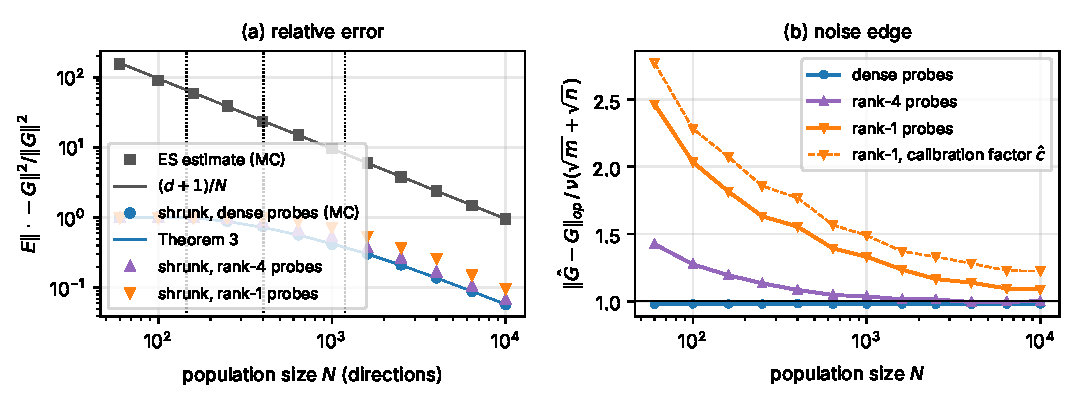
\includegraphics[width=\textwidth]{fig_risk.pdf}
\caption{$G$ is $80\times120$ with singular values $\propto(1,0.6,0.35)$; $d=9600$; 20 repetitions. (a) ES estimate and Algorithm~1; lines: $(d+1)/N$ and Theorem~\ref{thm:risk}; dotted: thresholds \eqref{eq:Nstar}. (b) Algorithm~1 with three kinds of probes. (c) Largest singular value of the noise $\Gh-G$ over the white-noise edge $\nu(\sqrt m+\sqrt n)$.}\label{fig:risk}
\end{figure}

\subsection{EGGROLL's rank-one probes make the noise heavier}
\begin{proposition}[Noise covariance for rank-$r$ probes]\label{prop:cov}
Assume (A1), one layer and rank-$r$ probes. Then
\[
N\,\E\big[(\Gh-G)(\Gh-G)^\top\big]=\Big(n+\frac2r\Big)\|G\|_F^2\,I_m+\Big(\frac{2n}{r}+1+\frac2r\Big)GG^\top\qquad(\text{dense probes: }n\|G\|_F^2I_m+GG^\top).
\]
\end{proposition}
\emph{In words:} the white part hardly depends on $r$, which is why the total error does not~[2]. The extra noise lies along the singular directions of $G$ itself, where the variance grows by the factor $1+\frac2r s_i^2/\|G\|_F^2$, up to $3$ for $r=1$; heavy tails add to this unless $N\gg\min(m,n)$ (Appendix~\ref{app:proofs}). So the top noise singular value is $2.5$ times the white-noise edge at $N=60$ and still $1.09$ times at $N=10^4$ (Figure~\ref{fig:risk}c), and Algorithm~1 with the white-noise edge is far worse than the zero estimate (Table~\ref{tab:flip}). Step 2 repairs this: random signs $\epsilon_j$ remove the signal from $\sum_j\epsilon_jy_jE_j$ (its mean is zero) but leave the noise essentially unchanged, so its top singular value measures the true noise edge at no cost. Rank-one probes then need about 2 to 2.5 times more probes than dense ones for the same error (Figure~\ref{fig:risk}b). \emph{A higher probe rank does not make the ES estimate more accurate, but it makes it easier to denoise.}

\subsection{Q3: a better estimate helps descent only in a window}\label{sec:q3}
\begin{proposition}[What a perfect estimate can gain]\label{prop:ceiling}
Assume (A1), dense probes, and a quadratic $f$ with Hessian $H\succeq0$ and $\ip{g}{Hg}>0$. Then, with $\Delta$ as in (Q3),
\[
\frac{\Delta(g)}{\Delta(\hat g)}=1+\frac{1+T}{N},\qquad T=\frac{\tr(H)\,\|g\|^2}{\ip{g}{Hg}},
\]
and every unbiased estimator $U$ satisfies $\Delta(U)\le\Delta(g)$.
\end{proposition}
\emph{In words:} the ES noise is spread over all directions and only meets the average curvature $\tr(H)/d$. If $H=hI$, then $T=d$ and the noise costs the full factor $d/N$. If $H$ has a few large eigenvalues and $g$ lies along them, $T$ is about the effective rank $\tr(H)/\lambda_{\max}(H)$ of~[14], possibly far below $d$: most of the noise falls in flat directions and costs nothing.

\textbf{A window.} Shrinkage changes the estimate only if $N>N^\star$ (Theorem~\ref{thm:risk}), and even removing all the noise gains only the factor $1+(1+T)/N$. So a low-rank prior can speed up descent only if $N^\star<N\lesssim T$. Two tests with rank-one probes:

\begin{figure}[t]
\centering
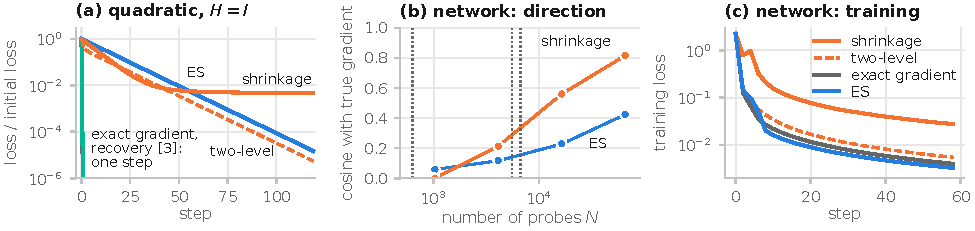
\includegraphics[width=\textwidth]{fig_descent.pdf}
\caption{Rank-one probes. (a) Quadratic, $H=I$, $N=4000$ per step, best stepsize per method. (b) Network after 100 gradient steps: cosine with the true gradient; line: $\sqrt{N/(N+d)}$; dotted: $N_1^\star$ of the three layers. (c) Network, $N=16384$, stepsize $1.2$.}\label{fig:descent}
\end{figure}

\emph{(a) Inside the window.} $f(W)=\frac12\|W-W^\star\|_F^2$ with a rank-3 target $W^\star\in\R^{200\times200}$ and $N=4000$ probes per step: $N_1^\star=311$ and $T=d=40000$, so the exact gradient is $11$ times better per step. ES needs 50 steps to reduce the loss 100-fold; the exact gradient needs one, and so does the recovery of~[3], since $N$ is $3.4$ times the number of degrees of freedom (Figure~\ref{fig:descent}a, Table~\ref{tab:recovery}). One-SVD shrinkage does not get there. Its first step removes $58\%$ of the loss (ES: $9\%$), but then it stalls, because it is biased: it returns only the detected directions, its error lies in new directions, and soon the residual $W_t-W^\star$ is spread over many directions, each near the detection level (Table~\ref{tab:stall}). Keeping the undetected part with a small weight (``two-level'', Appendix~\ref{app:exp}) avoids the stall but gains little (39 steps instead of 50). With a decaying spectrum instead ($T=210<N$, outside the window), the exact gradient is only $1.05$ times better and all methods are equally fast (Figure~\ref{fig:decaying}).

\emph{(b) A neural network: outside the window.} A tanh network $64$--$512$--$512$--$10$ on 256 images of the \texttt{digits} data ($d=300{,}032$), with rank-one probes on all three matrices and one shared scalar. The layer gradients have stable rank $\|G\|_F^2/s_1^2$ between 3 and 5; after 100 gradient steps the thresholds \eqref{eq:Nstar} of the three layers are $N_1^\star=6641$, $5554$, $630$, while $T$ stays between $80$ and $580$ along training (Table~\ref{tab:curv}): $N^\star>T$ in the two large layers, so the window is empty. Indeed, shrinkage improves the direction (at $N=16384$ the cosine with the true gradient rises from $0.23$ to $0.56$; Figure~\ref{fig:descent}b, Table~\ref{tab:nn}), but ES already trains as fast as the exact gradient at the same stepsize, and shrinkage, being biased, is slower than both (Figure~\ref{fig:descent}c, Table~\ref{tab:train}).

\section{Discussion and limitations}
\textbf{What the results establish.} \emph{Can a prior shrink the variance?} Without a preferred direction, no (Theorem~\ref{thm:nogo}). With a low-rank prior, yes: above a sharp, computable threshold, one SVD divides the error of a layer by up to $w/(2k)$, and the recovery of~[3] removes it from about $3k(m+n)$ probes on, in our test also with rank-one probes. \emph{Does it train faster?} Only if $N\lesssim T$. This is a condition on the loss, not on the estimator, so it limits every unbiased variance-reduction method for ES, including the baseline of~[2]. For ES training the right target is the curvature-weighted error $\ip{\tilde g-g}{H(\tilde g-g)}$, not $\|\tilde g-g\|^2$.

\textbf{Which assumptions matter.} Assumption (A1) needs a small radius $\sigma$. Theorems~\ref{thm:spike} and \ref{thm:risk} need dense probes and Theorem~\ref{thm:risk} is asymptotic; for rank-one probes we have only the covariance and simulations. Proposition~\ref{prop:ceiling} is for quadratics; the network is not quadratic, and at a fixed stepsize ES with fewer probes even reached a lower loss than the exact gradient (unexplained). We used one small network, one seed and plain updates.

\textbf{What remains unresolved.} A prior for the curvature-weighted error; Adam-type updates; the recovery of~[3] when matrices share scalars; and large models: for a $4096\times4096$ layer and $N=2^{18}$ probes, detection needs a direction with over $1.6\%$ of $\|g\|^2$, and~[14] suggests a small $T$ in fine-tuning.

\section{References and supporting material}
Code and reproduction details: Appendix~\ref{app:exp}. Use of AI (Claude, Anthropic): Appendix~\ref{app:ai}.

{\small
\begin{itemize}[leftmargin=2.2em,itemsep=0pt]
\item[{[1]}] B. Sarkar et al. Evolution strategies at the hyperscale. arXiv:2511.16652, 2025.
\item[{[2]}] E. C. Kaya, A. Hashemi. EGGROLL, unrolled: understanding and improving low-rank evolution strategies at scale. arXiv:2609.10980, 2026.
\item[{[3]}] S. Allen, C. Cherry, A. Eck, S. Becker, D. McKenzie. Gradient-free optimization for matrix functions. arXiv:2609.03170, 2026.
\item[{[4]}] M. Gavish, D. L. Donoho. Optimal shrinkage of singular values. \emph{IEEE Trans.\ Inf.\ Theory} 63(4), 2017.
\item[{[5]}] F. Benaych-Georges, R. R. Nadakuditi. The singular values and vectors of low rank perturbations of large rectangular random matrices. \emph{J. Multivariate Anal.} 111, 2012.
\item[{[6]}] B. Recht, M. Fazel, P. A. Parrilo. Guaranteed minimum-rank solutions of linear matrix equations via nuclear norm minimization. \emph{SIAM Review} 52(3), 2010.
\item[{[7]}] P. Jain, R. Meka, I. Dhillon. Guaranteed rank minimization via singular value projection. \emph{NeurIPS}, 2010.
\item[{[8]}] Y. Wang, S. Du, S. Balakrishnan, A. Singh. Stochastic zeroth-order optimization in high dimensions. \emph{AISTATS}, 2018.
\item[{[9]}] H. Cai, D. McKenzie, W. Yin, Z. Zhang. Zeroth-order regularized optimization (ZORO): approximately sparse gradients and adaptive sampling. \emph{SIAM J. Optim.} 32(2), 2022.
\item[{[10]}] N. Maheswaranathan, L. Metz, G. Tucker, D. Choi, J. Sohl-Dickstein. Guided evolutionary strategies: augmenting random search with surrogate gradients. \emph{ICML}, 2019.
\item[{[11]}] K. Choromanski, A. Pacchiano, J. Parker-Holder, Y. Tang, V. Sindhwani. From complexity to simplicity: adaptive ES-active subspaces for blackbox optimization. \emph{NeurIPS}, 2019.
\item[{[12]}] Y. Chen, Y. Zhang, L. Cao, K. Yuan, Z. Wen. Enhancing zeroth-order fine-tuning for language models with low-rank structures. \emph{ICLR}, 2025.
\item[{[13]}] J. Zhao, Z. Zhang, B. Chen, Z. Wang, A. Anandkumar, Y. Tian. GaLore: memory-efficient LLM training by gradient low-rank projection. \emph{ICML}, 2024.
\item[{[14]}] S. Malladi, T. Gao, E. Nichani, A. Damian, J. D. Lee, D. Chen, S. Arora. Fine-tuning language models with just forward passes. \emph{NeurIPS}, 2023.
\item[{[15]}] J. Tanner, K. Wei. Normalized iterative hard thresholding for matrix completion. \emph{SIAM J. Sci.\ Comput.} 35(5), 2013.
\item[{[16]}] R. Vershynin. Introduction to the non-asymptotic analysis of random matrices. In \emph{Compressed Sensing}, Cambridge Univ.\ Press, 2012.
\item[{[D]}] Our draft. \emph{Quadratic stability and excess risk of EGGROLL}, 2026.
\item[{[N]}] Our notes. \emph{Variance reduction for low-rank evolution strategies: curvature noise, perturbation radius, and factor design}, November 2026.
\end{itemize}}

\newpage
\appendix
\section{Proofs}\label{app:proofs}
We identify $g=(G_1,\dots,G_L)$ with a vector in $\R^d$ and use the Euclidean inner product.

\subsection{Proof of Theorem~\ref{thm:nogo}}
Condition on the probes, which are independent of $g$. Let $V=\mathrm{span}\{E_1,\dots,E_N\}$, $k=\dim V\le N$, and let $\Pi$ be the orthogonal projector on $V$. The data $y_j=\ip{E_j}{g}=\ip{E_j}{\Pi g}$ are a function of $\Pi g$. The map $Q=2\Pi-I$ is orthogonal, so $Qg\overset d=g$, and $\Pi Qg=\Pi g$, $(I-\Pi)Qg=-(I-\Pi)g$. Hence
\[
\big(\Pi g,\,(I-\Pi)g\big)\overset d=\big(\Pi g,\,-(I-\Pi)g\big),\qquad\text{so}\qquad\E\big[(I-\Pi)g\mid\Pi g\big]=0 .
\]
Let $\tilde g$ be any estimator; given the probes it is a (possibly randomized) function of $\Pi g$. Write $\tilde g-g=(\tilde g-\Pi g)-(I-\Pi)g$. The cross term has mean zero by the last display, so
\[
\E\|\tilde g-g\|^2=\E\|\tilde g-\Pi g\|^2+\E\|(I-\Pi)g\|^2\ \ge\ \E\|(I-\Pi)g\|^2=\Big(1-\frac kd\Big)\E\|g\|^2\ \ge\ 1-\frac Nd .
\]
The last equality uses $\E[gg^\top]=\frac1d\E\|g\|^2I$, which holds for rotation-invariant laws. The supremum over the unit sphere is at least the average over the uniform law on it. Equality holds for $\tilde g=\Pi g$ when $k=N$. The minimum-norm solution of $\ip{E_j}{h}=y_j$ is $\Pi g$, and the ridge estimator converges to it as $\lambda\to0$. \qed

\textbf{The plain ES estimate.} For i.i.d.\ probes with $\E\hat g=g$ and $\E\|\hat g\|^2=\kappa\|g\|^2$, $\min_a\E\|a\hat g-g\|^2=(1-1/\kappa)\|g\|^2$ at $a=1/\kappa$ [N, Prop.~9]. For dense probes $\kappa=1+(d+1)/N$ (also a consequence of Theorem~\ref{thm:spike}), so the fraction of $\|g\|^2$ that is explained is $1/\kappa=N/(N+d+1)$, against the optimum $N/d$.

\subsection{Proof of Theorem~\ref{thm:spike}}
Let $z_j=\ip{E_j}{u}$ and $E_j^\perp=E_j-z_ju$. Since $E_j$ is a standard Gaussian vector, $z_j\sim N(0,1)$, $E_j^\perp$ is Gaussian with covariance $I-uu^\top$, and the two are independent. With $y_j=\|g\|z_j$,
\[
\hat g=\frac{\|g\|}{N}\sum_jz_j\big(z_ju+E_j^\perp\big)=\alpha g+\frac{\|g\|}{N}\sum_jz_jE_j^\perp,\qquad\alpha=\frac1N\sum_jz_j^2 .
\]
Given $z=(z_1,\dots,z_N)$, the sum $\sum_jz_jE_j^\perp$ is Gaussian with mean zero and covariance $\|z\|^2(I-uu^\top)$. This is the law of $\|z\|(\Gamma-\ip{\Gamma}{u}u)$ for a standard Gaussian $\Gamma$. It depends on $z$ only through $\|z\|=\sqrt{N\alpha}$, so we can take $\Gamma$ independent of $z$. Then $\frac{\|g\|}{N}\sqrt{N\alpha}=\sqrt\alpha\,\|g\|/\sqrt N$. \qed

\emph{Check.} $\E\|\hat g-g\|^2=\|g\|^2\big[\E(\alpha-1)^2+\E\alpha\,\frac{d-1}{N}\big]=\frac{d+1}{N}\|g\|^2$, the known value [2].

\subsection{A bound for finite $N$}
\begin{proposition}\label{prop:finite}
Use dense probes, let $\mathrm{rank}(G_l)\le k$ and let $T_k$ be the truncation of the SVD to the top $k$ terms. Then always $\|T_k(\Gh_l)-G_l\|_F^2\le8k\|\Gh_l-G_l\|_\op^2$, and for every $t>0$, with probability at least $1-4e^{-t^2/2}$,
\[
\|\Gh_l-G_l\|_\op\le|\alpha-1|\,s_1(G_l)+\sqrt\alpha\,\frac{\|g\|}{\sqrt N}\big(\sqrt{m}+\sqrt{n}+2t\big),\qquad\E(\alpha-1)^2=\frac2N .
\]
\end{proposition}
\begin{proof}
$T_k(\Gh_l)-G_l$ has rank at most $2k$, so its Frobenius norm is at most $\sqrt{2k}$ times its operator norm. By the triangle inequality and Weyl's inequality, $\|T_k(\Gh_l)-G_l\|_\op\le\hat s_{k+1}+\|\Gh_l-G_l\|_\op\le2\|\Gh_l-G_l\|_\op$, because $s_{k+1}(G_l)=0$. For the second claim use Theorem~\ref{thm:spike}: $\Gh_l-G_l=(\alpha-1)G_l+\sqrt\alpha\,\nu(\Gamma_l-\ip{\Gamma}{u}u_l)$, where $u_l$ is the layer-$l$ block of $u$ and $\|u_l\|_\op\le1$. A Gaussian matrix satisfies $\|\Gamma_l\|_\op\le\sqrt m+\sqrt n+t$ with probability at least $1-2e^{-t^2/2}$ [16], and $|\ip{\Gamma}{u}|\le t$ with probability at least $1-2e^{-t^2/2}$.
\end{proof}
So, up to constants, the relative error of the truncated estimate is at most $8k\big(\sqrt m+\sqrt n\big)^2\|g\|^2/(N\|G_l\|_F^2)$, compared with $mn\|g\|^2/(N\|G_l\|_F^2)$ without truncation.

\subsection{Proof of Theorem~\ref{thm:risk} (reduction to [4, 5])}
By Theorem~\ref{thm:spike}, with $X=\sum_{i\le k}x_iu_iv_i^\top$ (the scaled SVD of $G$) and $W=\Gamma_l$,
\[
\frac{\Gh}{\sqrt\alpha\,\nu\sqrt n}=\sqrt\alpha\,X+\frac{W}{\sqrt n}-\frac{\ip{\Gamma}{u}}{\sqrt n}u_l .
\]
This is the spiked model $X'+W/\sqrt n$ of [4, 5] with $X'=\sqrt\alpha X-\ip{\Gamma}{u}u_l/\sqrt n$. As $N\to\infty$, $\alpha\to1$ almost surely and $|\ip{\Gamma}{u}|/\sqrt n\to0$, so $\|X'-X\|_\op\to0$ and $X'$ has rank at most $k+1$ with singular values converging to $x_1,\dots,x_k,0$. For the model $X+W/\sqrt n$, [5, Theorems 2.8--2.9] give, for $x_i>\beta^{1/4}$,
\[
\hat s_i\to\sqrt{\Big(x_i+\frac1{x_i}\Big)\Big(x_i+\frac\beta{x_i}\Big)},\qquad
\ip{\hat u_i}{u_i}^2\to c_i^2=\frac{x_i^4-\beta}{x_i^4+\beta x_i^2},\qquad
\ip{\hat v_i}{v_i}^2\to\tilde c_i^2=\frac{x_i^4-\beta}{x_i^4+x_i^2},
\]
and for $x_i\le\beta^{1/4}$, $\hat s_i\to1+\sqrt\beta$ with asymptotically no correlation between the singular vectors. [4, Section IV] shows that the loss of a shrinker with values $\eta_i$ then converges to $\sum_i(x_i^2+\eta_i^2-2x_i\eta_ic_i\tilde c_i)$, that the minimizer is $\eta_i=x_ic_i\tilde c_i$, and that this equals the function $\eta(\hat s_i)$ of \eqref{eq:shr}. The minimum is $x_i^2(1-c_i^2\tilde c_i^2)=R(x_i)$, and a non-detected spike contributes $x_i^2$. Since these limits are continuous in the spike strengths, they are not changed by replacing $X$ with $X'$, nor by the factor $\sqrt\alpha\to1$ in the scaling. The condition $x_i>\beta^{1/4}$ reads $s_i^2N/(\|g\|^2n)>\sqrt{m/n}$, which is \eqref{eq:Nstar}. For $x\to\infty$, $(x^4-\beta)^2/(x^2(x^2+\beta)(x^2+1))=x^2-(1+\beta)+O(x^{-2})$. \qed

We state this as a reduction: the only new step is Theorem~\ref{thm:spike}, which puts the ES estimate into the model of [4, 5]. We did not re-derive the limits of [4, 5]; Figure~\ref{fig:risk}(a) checks the final formula numerically.

\subsection{Proof of Proposition~\ref{prop:cov}}
One probe gives $\Gh_1=yE$ with $E=AB^\top/\sqrt r$ and $y=\ip{E}{G}=\ip{M}{B}/\sqrt r$, $M=G^\top A\in\R^{n\times r}$. Since $\E\Gh_1=G$ and the $N$ terms are independent, $N\,\E[(\Gh-G)(\Gh-G)^\top]=\E[\Gh_1\Gh_1^\top]-GG^\top$. Now $\Gh_1\Gh_1^\top=\frac1{r^2}\ip{M}{B}^2AB^\top BA^\top$. Given $A$, Isserlis' formula for the Gaussian matrix $B$ gives
\[
\E_B\big[\ip{M}{B}^2B^\top B\big]=n\|M\|_F^2I_r+2M^\top M .
\]
With $S=GG^\top$, $\|M\|_F^2=\tr(A^\top SA)$ and $M^\top M=A^\top SA$, so $\E[\Gh_1\Gh_1^\top]=\frac1{r^2}\E\big[n\tr(A^\top SA)AA^\top+2AA^\top SAA^\top\big]$. Let $a_1,\dots,a_r$ be the columns of $A$. Using $\E[(a^\top Sa)aa^\top]=\tr(S)I+2S$ for one column and independence for two different columns,
\[
\E\big[\tr(A^\top SA)AA^\top\big]=r^2\tr(S)I+2rS,\qquad\E\big[AA^\top SAA^\top\big]=r(r+1)S+r\tr(S)I .
\]
Together, $\E[\Gh_1\Gh_1^\top]=(n+\frac2r)\tr(S)I+(\frac{2n}r+2+\frac2r)S$; subtract $GG^\top$ and note $\tr(S)=\|G\|_F^2$. The other side follows by exchanging the roles of $A$ and $B$. For dense probes, $\E[\ip{E}{G}^2EE^\top]=n\|G\|_F^2I+2GG^\top$ by Isserlis' formula. \qed

We checked the formula by Monte Carlo ($6\times9$, rank-2 $G$, $4\cdot10^5$ samples): the largest entrywise deviation, relative to the largest entry, is below $1\%$ for $r=1,2,8$.

\subsection{Proof of Proposition~\ref{prop:ceiling}}
For a quadratic, $f(W-\eta D)-f(W)=-\eta\ip{g}{D}+\frac{\eta^2}2\ip{D}{HD}$. For $D=\hat g$ with dense probes, $\E\hat g=g$ and
\[
\E\ip{\hat g}{H\hat g}=\Big(1-\frac1N\Big)\ip{g}{Hg}+\frac1N\E\big[\ip{g}{E}^2\ip{E}{HE}\big]=\Big(1+\frac1N\Big)\ip{g}{Hg}+\frac1N\tr(H)\|g\|^2,
\]
by independence of the probes and Isserlis' formula $\E[\ip{g}{E}^2\ip{E}{HE}]=\tr(H)\|g\|^2+2\ip{g}{Hg}$. Minimizing $-\eta\|g\|^2+\frac{\eta^2}2Q$ over $\eta$ gives the decrease $\|g\|^4/(2Q)$; $Q=\E\ip{\hat g}{H\hat g}$ for ES and $Q=\ip{g}{Hg}$ for the exact gradient. \qed

The second-moment identity is from our notes [N, Prop.~10]. For rank-one probes and Kronecker $H$ the term $\tr(H)\|g\|^2$ gets small corrections given there.

\section{Use of AI}
We used Claude (Anthropic) to explore ideas, to derive and check proofs, to write the code and to draft the text. The question, the earlier draft [D] and notes [N], and the final checking are ours.

\section{Experiments: details and further results}\label{app:exp}
All code is in the repository (\texttt{code/}); every number in this report is produced by the scripts named below, with fixed seeds. Only \texttt{numpy} is needed (and \texttt{scikit-learn} for the data).

\textbf{Figure~\ref{fig:risk} (\texttt{exp\_risk.py}).} $G=U\,\mathrm{diag}(s)V^\top$ with Haar factors and $s\propto(1,0.6,0.35)$. ``Shrunk'' is \eqref{eq:shr} with $\hat\nu^2=\frac1{N^2}\sum_jy_j^2$; for rank-1 and rank-4 probes with the sign-flip factor $\hat c$. Table~\ref{tab:flip} shows that the calibration is necessary for low-rank probes and costs little for dense ones.

\begin{table}[H]
\centering\small
\caption{Relative error of the shrunk estimate without and with sign-flip calibration (setting of Figure~\ref{fig:risk}). Values above 1 are worse than the zero estimate.}\label{tab:flip}
\begin{tabular}{lcccccc}
\toprule
$N$ & 60 & 160 & 400 & 1000 & 2500 & 10000\\
\midrule
dense probes, no calibration & 1.00 & 0.99 & 0.75 & 0.42 & 0.21 & 0.058\\
dense probes, calibrated & 1.00 & 1.00 & 0.83 & 0.47 & 0.23 & 0.059\\
rank-4 probes, no calibration & 21.7 & 3.41 & 1.05 & 0.52 & 0.25 & 0.068\\
rank-4 probes, calibrated & 1.00 & 1.00 & 0.86 & 0.54 & 0.27 & 0.068\\
rank-1 probes, no calibration & 70.9 & 15.1 & 4.16 & 1.14 & 0.39 & 0.097\\
rank-1 probes, calibrated & 1.00 & 1.00 & 0.99 & 0.73 & 0.37 & 0.097\\
\midrule
Theorem~\ref{thm:risk} (dense) & 1.00 & 0.99 & 0.73 & 0.42 & 0.21 & 0.058\\
plain ES, $(d+1)/N$ & 160 & 60 & 24 & 9.6 & 3.8 & 0.96\\
\bottomrule
\end{tabular}
\end{table}

\textbf{Figure~\ref{fig:descent} (\texttt{exp\_descent.py}).} $f(W)=\frac12\ip{W-W^\star}{L(W-W^\star)R}$ with diagonal $L,R$; $W^\star$ has singular values $(3,2,1)$. Stepsize grids: powers of two around $1/\kappa$ for ES and around $1$ for the shrinkage methods; the best final loss is shown. Steps to reach $10^{-2}$ of the initial loss for $H=I$: exact gradient 1, ES 50, two-level 39, shrinkage only 37 (but it stalls at $4.5\cdot10^{-3}$). Steps to $10^{-4}$: ES 99, two-level 89. Table~\ref{tab:stall} shows the stall.

\begin{table}[H]
\centering\small
\caption{Shrinkage only, stepsize 1, $H=I$, rank-one probes, one run. ``Top share'' is $s_1^2/\|G\|_F^2$ of the current gradient $G=W_t-W^\star$. ``Error'' is the relative error of the shrunk estimate at this step.}\label{tab:stall}
\begin{tabular}{lccccccccc}
\toprule
step & 0 & 1 & 2 & 3 & 4 & 6 & 8 & 10\\
\midrule
loss & 7.00 & 2.99 & 1.77 & 1.52 & 1.18 & 0.95 & 0.86 & 0.77\\
top share & 0.64 & 0.27 & 0.22 & 0.21 & 0.19 & 0.15 & 0.12 & 0.12\\
directions kept & 2 & 4 & 2 & 3 & 2 & 1 & 1 & 1\\
error & 0.43 & 0.59 & 0.86 & 0.78 & 0.89 & 0.96 & 0.98 & 0.97\\
\bottomrule
\end{tabular}
\end{table}

\textbf{Figure~\ref{fig:nn} (\texttt{exp\_nn\_wide.py}).} Network $64$--$512$--$512$--$10$, tanh, Gaussian initialization, cross-entropy on a fixed batch of 256 standardized \texttt{digits} images. The directional derivatives are exact, $y_j=\sum_la_{j,l}^\top G_lb_{j,l}$ with $G_l$ from backpropagation; this is the limit $\sigma\to0$ of an antithetic pair. In the small network, antithetic finite differences with $\sigma=10^{-3}$ differ from the exact values by $0.015\%$ in relative $\ell_2$ norm, by $1.3\%$ for $\sigma=10^{-2}$ and by $60\%$ for $\sigma=0.1$ (\texttt{check\_fd.py}); so the model \eqref{eq:model} needs a small radius.

\begin{table}[H]
\centering\small
\caption{Network $64$--$512$--$512$--$10$ after 100 gradient steps (loss $0.012$). Relative error per layer: plain ES / shrunk (measured, rank-one probes, calibrated, one draw) / Theorem~\ref{thm:risk} (dense probes).}\label{tab:nn}
\begin{tabular}{lccccc}
\toprule
layer (shape) & $N_1^\star$ & $N=1024$ & $N=4096$ & $N=16384$ & $N=65536$\\
\midrule
1 ($512\times64$) & 6641 & 257 / 1.00 / 1.00 & 65 / 1.00 / 1.00 & 16 / 0.95 / 0.92 & 3.9 / 0.64 / 0.57\\
2 ($512\times512$) & 5554 & 636 / 1.00 / 1.00 & 164 / 1.00 / 1.00 & 40 / 0.91 / 0.84 & 10 / 0.47 / 0.41\\
3 ($10\times512$) & 630 & 12 / 1.00 / 0.98 & 2.9 / 0.91 / 0.73 & 0.75 / 0.43 / 0.37 & 0.19 / 0.14 / 0.13\\
\bottomrule
\end{tabular}
\end{table}
The per-layer errors stay large in the two wide layers even when the cosine of the whole gradient is high: the estimate keeps the top directions and drops the rest, and the last layer carries about half of $\|g\|^2$.

\textbf{Small network (\texttt{exp\_nn.py}).} $64$--$96$--$96$--$10$, $d=16320$, $N=1024$ antithetic pairs with $\sigma=10^{-3}$ (true finite differences). After 300 gradient steps, $N_1^\star=2147$, $2216$, $366$. Shrinkage returns zero for layers 1 and 2 and has relative error $0.92$ in layer 3 (Theorem~\ref{thm:risk}: $1.00$, $1.00$, $0.81$). The cosine of the whole gradient is $0.24$ for ES and $0.29$ for two-level shrinkage.

TRAINTABLEPLACEHOLDER

\textbf{Iterated shrinkage on the same evaluations (\texttt{shrink.py}, \texttt{iterated\_shrink}).} We iterate $G^{(k+1)}=\mathcal S\big(G^{(k)}+\frac1N\sum_j(y_j-\ip{E_j}{G^{(k)}})E_j\big)$ with the noise level re-estimated from the residuals. This is singular value projection [7] with a data-driven threshold. For a $200\times200$ rank-3 gradient ($k(m+n)=1200$), one run each:

\begin{table}[H]
\centering\small
\caption{Relative error; ``iterated'' after 5 / 20 / 60 passes.}
\begin{tabular}{lcccc}
\toprule
 & $N=1000$ & $N=2000$ & $N=4000$ & $N=8000$\\
\midrule
rank-1 probes, one pass & 0.92 & 0.73 & 0.45 & 0.24\\
rank-1 probes, iterated & 0.89 / 0.86 / 0.87 & 0.73 / 1.00 / 1.00 & 0.45 / 1.00 / 1.00 & 0.06 / 0.09 / 0.09\\
rank-8 probes, one pass & 0.80 & 0.47 & 0.29 & 0.15\\
rank-8 probes, iterated & 0.67 / 0.47 / 0.78 & 0.50 / 0.75 / 0.82 & 0.08 / 0.66 / 0.46 & 0.003 / 0.000 / 0.000\\
\bottomrule
\end{tabular}
\end{table}
With rank-8 probes and $N=8000$ the gradient is recovered exactly from the same evaluations, as in [3]. Closer to $k(m+n)$ the plain iteration is unstable. We report this as an open point, not as a method.

\end{document}
